\chapter{O mol e a massa molar}\label{ch:g10:the-mole}

No fim do dia, um banco não conta as suas moedas uma por uma: ele as
pesa. Se uma moeda tem massa de \qty{7.5}{g}, um saco de moedas com massa
de \qty{7.5}{kg} contém mil moedas, e a balança fez a contagem. Os
químicos enfrentam o mesmo problema com os \omterm{def:g7:atoms-and-molecules:atom}{átomos}, só que muito pior: uma
colherada de água contém mais \omterm{def:g7:atoms-and-molecules:molecule}{moléculas} do que há grãos de areia em
todas as praias de um litoral. Eles o resolvem do mesmo jeito, pesando,
e o saco que eles usam contém
\num{602214076000000000000000} entidades. Este capítulo define esse saco,
o \omterm{def:g10:the-mole:amount}{mol}, e mostra como passar de uma massa lida numa balança a um número
de \omterm{def:g7:atoms-and-molecules:atom}{átomos} ou de \omterm{def:g7:atoms-and-molecules:molecule}{moléculas}.

\begin{recall}
A massa de um \omterm{def:g7:atoms-and-molecules:atom}{átomo} está concentrada no seu \omterm{def:g9:inside-the-atom:nucleus}{núcleo}; um \omterm{def:g9:inside-the-atom:proton}{próton} e um
\omterm{def:g9:inside-the-atom:proton}{nêutron} têm, cada um, massa de cerca de \qty{1.67e-27}{kg}, de modo que
um \omterm{def:g7:atoms-and-molecules:atom}{átomo} de \omterm{def:g9:inside-the-atom:atomic-number}{número de massa} $A$ tem massa de cerca de
$A \times \qty{1.67e-27}{kg}$. Os números muito grandes e muito pequenos
são escritos em notação científica
(\cref{ch:g9:inside-the-atom}). Uma \omterm{def:g7:atoms-and-molecules:formula}{fórmula química} dá o número de
\omterm{def:g7:atoms-and-molecules:atom}{átomos} de cada elemento numa \omterm{def:g7:atoms-and-molecules:molecule}{molécula} (\cref{ch:g7:atoms-and-molecules}).
\end{recall}

\begin{omfigure}
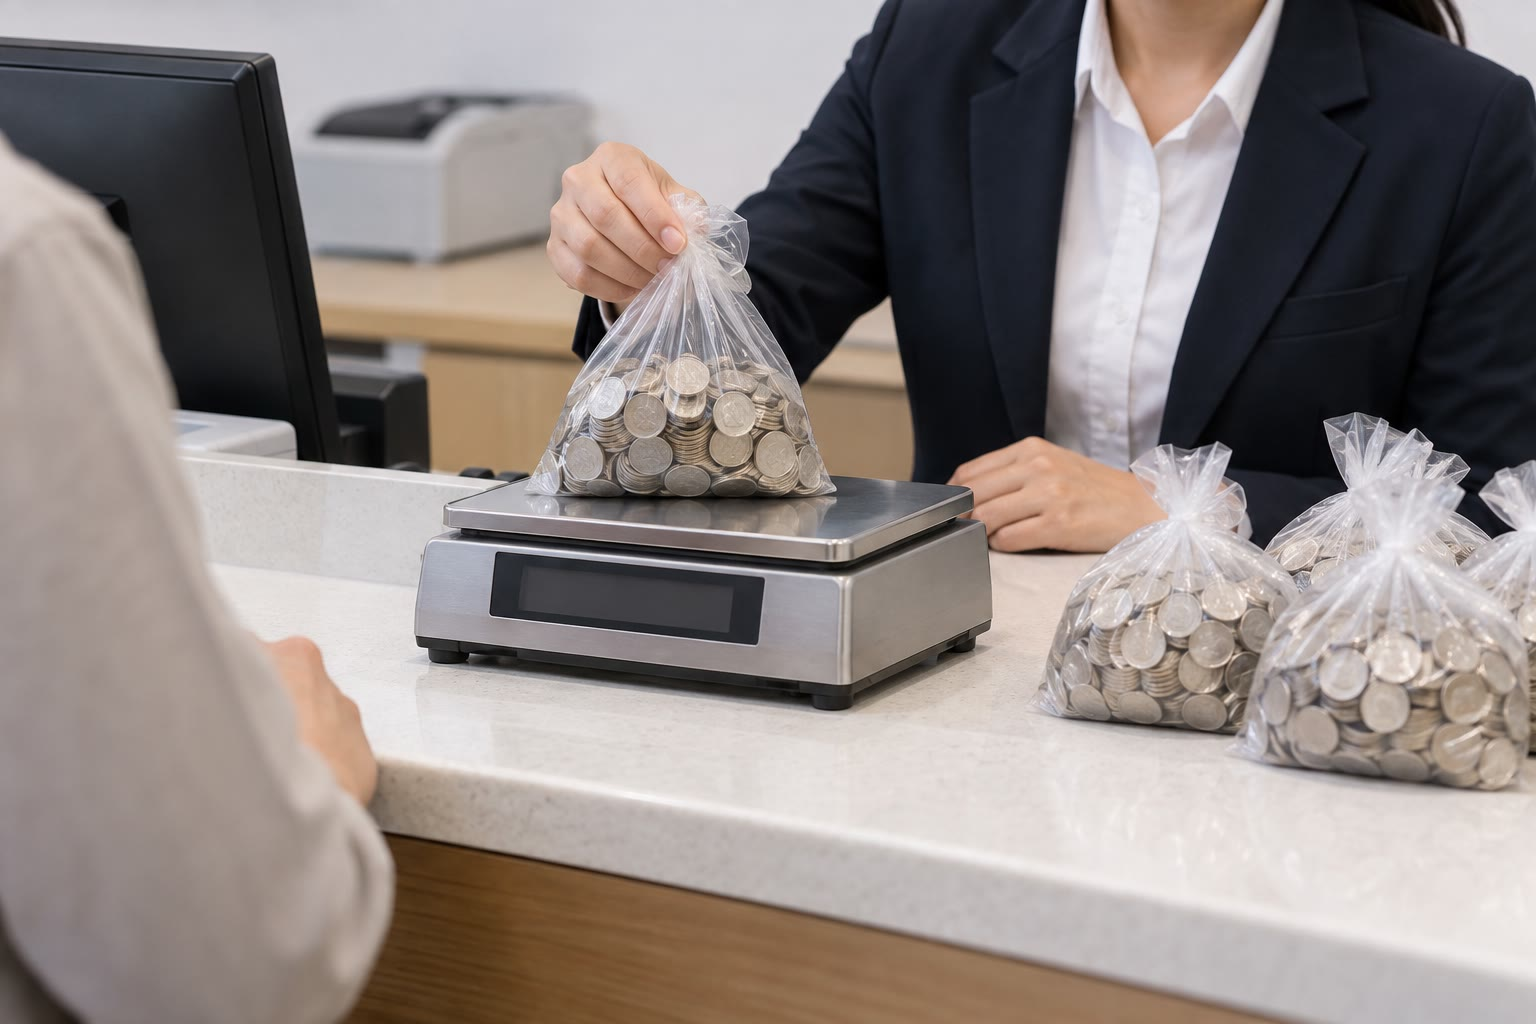
\includegraphics[width=0.55\linewidth]{images/book1/ai/g10-bank-coins.jpg}

{\small Um banco conta as moedas pesando-as. Os químicos contam os \omterm{def:g7:atoms-and-molecules:atom}{átomos}
do mesmo jeito.}
\end{omfigure}

\section{Contar pesando}

\begin{example}[Um saco de moedas]\label{ex:g10:the-mole:coins}
Uma moeda tem massa de \qty{7.5}{g}. Um saco dessas moedas tem massa de
\qty{1.80}{kg}, isto é, \qty{1800}{g}, sem contar a massa do próprio
saco. Ele contém
\[
  \frac{\qty{1800}{g}}{\qty{7.5}{g}} = 240 \text{ moedas.}
\]
Para contar, o banco divide a massa total pela massa de uma moeda.
\end{example}

\begin{example}[Uma colherada de água]\label{ex:g10:the-mole:spoon}
Uma \omterm{def:g7:atoms-and-molecules:molecule}{molécula} de água, \ce{H2O}, tem $2 + 16 = 18$ \omterm{def:g9:inside-the-atom:proton}{núcleons} (os \omterm{def:g7:atoms-and-molecules:atom}{átomos} de
oxigênio-16 e de hidrogênio-1 formam quase toda a água natural), por isso
a sua massa é de cerca de
$18 \times \qty{1.67e-27}{kg} = \qty{3.0e-26}{kg}$, ou
\qty{3.0e-23}{g}. Uma colherada de \qty{5.0}{g} de água contém, portanto,
\[
  \frac{\qty{5.0}{g}}{\qty{3.0e-23}{g}} \approx \num{1.7e23}
  \text{ moléculas.}
\]
A divisão funciona como para as moedas, mas a resposta é um número que
ninguém consegue imaginar. Os químicos precisam de um pacote de \omterm{def:g7:atoms-and-molecules:atom}{átomos}
adaptado às amostras do laboratório.
\end{example}

\begin{definition}[Quantidade de matéria e mol]\label{def:g10:the-mole:amount}
% ledger: const:NA
A \emph{quantidade de matéria}\index{quantidade de materia@quantidade de matéria} $n$ de uma
amostra conta as entidades que ela contém (\omterm{def:g7:atoms-and-molecules:atom}{átomos}, \omterm{def:g7:atoms-and-molecules:molecule}{moléculas} ou \omterm{def:g9:ions:ion}{íons},
especificados a cada vez). A sua unidade é o \emph{mol}\index{mol},
símbolo \si{mol}: um mol contém exatamente \num{6.02214076e23}
entidades.
\end{definition}

\begin{remark}[Uma dúzia, uma resma, um mol]\label{rem:g10:the-mole:dozen}
O \omterm{def:g10:the-mole:amount}{mol} é uma unidade de contagem, como uma dúzia de ovos (12) ou uma resma
de papel (500 folhas), só que muito maior. ``Dois \omterm{def:g10:the-mole:amount}{mols} de \omterm{def:g7:atoms-and-molecules:molecule}{moléculas} de
água'' quer dizer $2 \times \num{6.02214076e23} = \num{1.20e24}$
\omterm{def:g7:atoms-and-molecules:molecule}{moléculas}, assim como ``duas dúzias de ovos'' quer dizer 24 ovos. Diga
sempre que entidades são contadas: um \omterm{def:g10:the-mole:amount}{mol} de \emph{\omterm{def:g7:atoms-and-molecules:molecule}{moléculas}} de
oxigênio \ce{O2} contém dois \omterm{def:g10:the-mole:amount}{mols} de \emph{\omterm{def:g7:atoms-and-molecules:atom}{átomos}} de oxigênio.
\end{remark}

\begin{history}[A hipótese de Avogadro, 1811]
Em 1811, o físico Amedeo Avogadro propôs que volumes iguais de gases
diferentes, à mesma temperatura e à mesma pressão, contêm o mesmo número
de partículas. Ele também entendeu que um gás como o oxigênio é formado
por \omterm{def:g7:atoms-and-molecules:molecule}{moléculas} de dois \omterm{def:g7:atoms-and-molecules:atom}{átomos}. A sua ideia foi deixada de lado durante
quase cinquenta anos, até que Stanislao Cannizzaro a usou, em 1860, para
obter um conjunto coerente de pesos atômicos. A constante que conta as
entidades de um \omterm{def:g10:the-mole:amount}{mol} recebeu mais tarde o nome de Avogadro; ele nunca
conheceu o seu valor.
\end{history}

\begin{omfigure}
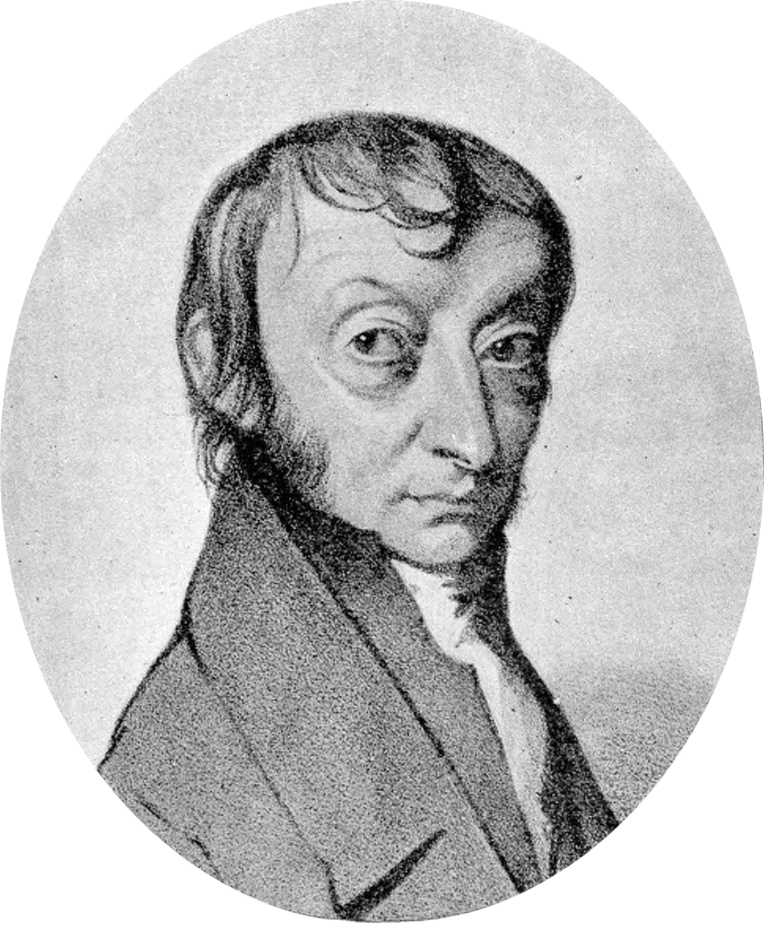
\includegraphics[width=0.26\linewidth]{images/book1/avogadro.jpg}

{\small Amedeo Avogadro (1776--1856).}
\end{omfigure}

\section{A constante de Avogadro}

\begin{definition}[Constante de Avogadro]\label{def:g10:the-mole:avogadro}
% ledger: const:NA
A \emph{constante de Avogadro}\index{constante de Avogadro} $N_A$ é o
número de entidades por \omterm{def:g10:the-mole:amount}{mol}:
\[
  N_A = \qty{6.02214076e23}{mol^{-1}} .
\]
O seu valor é exato, fixado por definição. Nos cálculos, ele é
arredondado para \qty{6.02e23}{mol^{-1}}.
\end{definition}

\begin{proposition}[Número de entidades e quantidade de matéria]\label{prop:g10:the-mole:number}
Uma amostra que contém $N$ entidades contém a \omterm{def:g10:the-mole:amount}{quantidade de matéria}
\[
  n = \frac{N}{N_A}, \qquad\text{isto é,}\qquad N = n \times N_A .
\]
\end{proposition}

\begin{proof}
Cada \omterm{def:g10:the-mole:amount}{mol} contém $N_A$ entidades, logo $n$ \omterm{def:g10:the-mole:amount}{mols} contêm $n \times N_A$
entidades; dividindo por $N_A$, obtém-se $n$.
\end{proof}

\begin{example}[Moléculas e mols]\label{ex:g10:the-mole:convert}
Uma amostra contém \num{1.5e24} \omterm{def:g7:atoms-and-molecules:molecule}{moléculas} de dióxido de carbono. A sua
quantidade de dióxido de carbono é
$n = \num{1.5e24} / \qty{6.02e23}{mol^{-1}} = \qty{2.5}{mol}$.
Inversamente, \qty{0.20}{mol} de ferro contêm
$N = \qty{0.20}{mol} \times \qty{6.02e23}{mol^{-1}} = \num{1.2e23}$
\omterm{def:g7:atoms-and-molecules:atom}{átomos} de ferro.
\end{example}

\begin{remark}[De onde vem o número]\label{rem:g10:the-mole:origin}
Durante mais de cinquenta anos, o \omterm{def:g10:the-mole:amount}{mol} foi definido como o número de
\omterm{def:g7:atoms-and-molecules:atom}{átomos} em exatamente \qty{12}{g} de carbono-12, e $N_A$ tinha de ser
medido. Desde 2019, o próprio número foi fixado, o que faz do \omterm{def:g10:the-mole:amount}{mol} uma
contagem pura. A definição antiga e a nova concordam com uma diferença
menor que uma parte em cem milhões, de modo que doze gramas de
carbono-12 continuam contendo um \omterm{def:g10:the-mole:amount}{mol} de \omterm{def:g7:atoms-and-molecules:atom}{átomos}, como a seção seguinte
verifica.
\end{remark}

\section{A massa molar}

\begin{definition}[Massa molar]\label{def:g10:the-mole:molar-mass}
A \emph{massa molar}\index{massa molar} $M$ de uma \omterm{def:g6:pure-substances-and-mixtures:species}{espécie química} é a
massa de um \omterm{def:g10:the-mole:amount}{mol} das suas entidades, em gramas por \omterm{def:g10:the-mole:amount}{mol} (\si{g/mol}). A
massa molar de um elemento, tomada sobre a sua \omterm{def:g6:pure-substances-and-mixtures:mixture}{mistura} natural de
\omterm{def:g9:inside-the-atom:isotope}{isótopos}, é a sua \emph{massa molar atômica}\index{massa molar atomica@massa molar atômica};
ela vem impressa na \omterm{def:g9:periodic-table-first-look:periodic-table}{tabela periódica}.
\end{definition}

\begin{example}[Um mol de átomos de carbono]\label{ex:g10:the-mole:carbon}
% ledger: const:NA, const:u
Um \omterm{def:g7:atoms-and-molecules:atom}{átomo} de carbono-12 tem massa de cerca de
$12 \times \qty{1.67e-27}{kg} = \qty{2.00e-26}{kg}$. Um \omterm{def:g10:the-mole:amount}{mol} deles
tem massa de
\[
  \qty{2.00e-26}{kg} \times \num{6.02e23} = \qty{1.20e-2}{kg}
  = \qty{12.0}{g}.
\]
O \omterm{def:g10:the-mole:amount}{mol} foi escolhido de modo que a \omterm{def:g10:the-mole:molar-mass}{massa molar} de um \omterm{def:g7:atoms-and-molecules:atom}{átomo}, em gramas por
\omterm{def:g10:the-mole:amount}{mol}, seja próxima do seu \omterm{def:g9:inside-the-atom:atomic-number}{número de massa}: cerca de \qty{1}{g/mol} para o
hidrogênio, \qty{12}{g/mol} para o carbono, \qty{16}{g/mol} para o
oxigênio.
\end{example}

\begin{omfigure}
% ledger: aw:H, aw:C, aw:N, aw:O, aw:Na, aw:Mg, aw:Al, aw:Si, aw:S, aw:Cl, aw:K, aw:Ca, aw:Fe, aw:Cu, aw:Zn, aw:Au (rounded to 0.1)
\begin{tabular}{lcr@{\qquad}lcr}
\hline
elemento & símbolo & $M$ (\si{g/mol}) & elemento & símbolo & $M$ (\si{g/mol}) \\
\hline
hidrogênio & \ce{H}  & 1.0  & silício   & \ce{Si} & 28.1 \\
carbono    & \ce{C}  & 12.0 & enxofre   & \ce{S}  & 32.1 \\
nitrogênio & \ce{N}  & 14.0 & cloro     & \ce{Cl} & 35.5 \\
oxigênio   & \ce{O}  & 16.0 & potássio  & \ce{K}  & 39.1 \\
sódio      & \ce{Na} & 23.0 & cálcio    & \ce{Ca} & 40.1 \\
magnésio   & \ce{Mg} & 24.3 & ferro     & \ce{Fe} & 55.8 \\
alumínio   & \ce{Al} & 27.0 & cobre     & \ce{Cu} & 63.5 \\
           &         &      & ouro      & \ce{Au} & 197.0 \\
\hline
\end{tabular}\par\medskip

{\small \omterm{def:g10:the-mole:molar-mass}{Massas molares atômicas} de elementos comuns, arredondadas a
\qty{0.1}{g/mol}. São os valores usados neste livro.}
\end{omfigure}

\begin{remark}[Por que o cloro tem 35.5]\label{rem:g10:the-mole:chlorine}
% ledger: iso:Cl35, iso:Cl37
O cloro natural é uma \omterm{def:g6:pure-substances-and-mixtures:mixture}{mistura} de dois \omterm{def:g9:inside-the-atom:isotope}{isótopos}: cerca de três quartos
dos seus \omterm{def:g7:atoms-and-molecules:atom}{átomos} são de cloro-35, um quarto de cloro-37
(\cref{ch:g9:inside-the-atom}). A sua \omterm{def:g10:the-mole:molar-mass}{massa molar atômica} é a média
ponderada por essas proporções, que fica entre 35 e 37:
\qty{35.5}{g/mol}. É por isso que algumas \omterm{def:g10:the-mole:molar-mass}{massas molares atômicas} estão
longe de números inteiros.
\end{remark}

\begin{proposition}[Massa molar de uma molécula]\label{prop:g10:the-mole:sum}
A \omterm{def:g10:the-mole:molar-mass}{massa molar} de uma \omterm{def:g7:atoms-and-molecules:molecule}{molécula} é a soma das \omterm{def:g10:the-mole:molar-mass}{massas molares atômicas} de
todos os seus \omterm{def:g7:atoms-and-molecules:atom}{átomos}, cada um contado tantas vezes quantas aparece na
fórmula. A mesma regra dá a \omterm{def:g10:the-mole:molar-mass}{massa molar} de um sólido iônico a partir da
sua unidade de fórmula.
\end{proposition}

\begin{proof}
Um \omterm{def:g10:the-mole:amount}{mol} de \omterm{def:g7:atoms-and-molecules:molecule}{moléculas} \ce{A_xB_y} contém $x$ \omterm{def:g10:the-mole:amount}{mols} de \omterm{def:g7:atoms-and-molecules:atom}{átomos} \ce{A} e $y$
\omterm{def:g10:the-mole:amount}{mols} de \omterm{def:g7:atoms-and-molecules:atom}{átomos} \ce{B}, e mais nada; a sua massa é a soma das massas
deles, $x\,M(\ce{A}) + y\,M(\ce{B})$.
\end{proof}

\begin{example}[Três massas molares]\label{ex:g10:the-mole:three}
% ledger: aw:H, aw:C, aw:O, aw:Na, aw:Cl
\begin{align*}
  M(\ce{H2O}) &= 2 \times 1.0 + 16.0 = \qty{18.0}{g/mol},\\
  M(\ce{NaCl}) &= 23.0 + 35.5 = \qty{58.5}{g/mol},\\
  M(\ce{C12H22O11}) &= 12 \times 12.0 + 22 \times 1.0 + 11 \times 16.0
     = \qty{342.0}{g/mol}.
\end{align*}
A última é a sacarose, o açúcar de mesa.
\end{example}

\section{Da massa à quantidade de matéria, e de volta}

\begin{proposition}[Massa e quantidade de matéria]\label{prop:g10:the-mole:mass}
Uma amostra de massa $m$ de uma espécie de \omterm{def:g10:the-mole:molar-mass}{massa molar} $M$ contém a
\omterm{def:g10:the-mole:amount}{quantidade de matéria}
\[
  n = \frac{m}{M}, \qquad\text{isto é,}\qquad m = n \times M .
\]
Com $m$ em gramas e $M$ em gramas por \omterm{def:g10:the-mole:amount}{mol}, $n$ fica em \omterm{def:g10:the-mole:amount}{mols}.
\end{proposition}

\begin{proof}
Cada \omterm{def:g10:the-mole:amount}{mol} tem massa $M$, logo $n$ \omterm{def:g10:the-mole:amount}{mols} têm massa $n \times M$; é a
contagem de moedas do banco, com o \omterm{def:g10:the-mole:amount}{mol} no papel da moeda.
\end{proof}

\begin{method}[De uma massa a um número de entidades]\label{met:g10:the-mole:mass-to-number}
\begin{enumerate}
  \item Escreva a fórmula da espécie e calcule a sua \omterm{def:g10:the-mole:molar-mass}{massa molar} $M$ a
        partir da tabela.
  \item Converta a massa em gramas, se necessário, e depois $n = m / M$.
  \item Se o número de entidades for pedido, $N = n \times N_A$.
  \item Verifique a ordem de grandeza: alguns gramas de uma \omterm{def:g7:atoms-and-molecules:molecule}{molécula}
        pequena são da ordem de um décimo de \omterm{def:g10:the-mole:amount}{mol}, umas $10^{22}$ a
        $10^{23}$ entidades.
\end{enumerate}
\end{method}

\begin{omfigure}
\begin{tikzpicture}[font=\small, box/.style={draw=omDef, very thick,
    fill=omDef!8, rounded corners=3pt, minimum width=2.9cm,
    minimum height=1.1cm, align=center}]
  \node[box] (m) at (0,0) {massa $m$\\[1pt] (\si{g})};
  \node[box] (n) at (5,0) {quantidade $n$\\[1pt] (\si{mol})};
  \node[box] (N) at (10,0) {número $N$\\[1pt] de entidades};
  \draw[-{Stealth[length=7pt]}, thick, omProp] ([yshift=4pt]m.east)
    -- node[above] {$\div M$} ([yshift=4pt]n.west);
  \draw[-{Stealth[length=7pt]}, thick, omProp] ([yshift=-4pt]n.west)
    -- node[below] {$\times M$} ([yshift=-4pt]m.east);
  \draw[-{Stealth[length=7pt]}, thick, omProp] ([yshift=4pt]n.east)
    -- node[above] {$\times N_A$} ([yshift=4pt]N.west);
  \draw[-{Stealth[length=7pt]}, thick, omProp] ([yshift=-4pt]N.west)
    -- node[below] {$\div N_A$} ([yshift=-4pt]n.east);
\end{tikzpicture}

{\small A \omterm{def:g10:the-mole:amount}{quantidade de matéria} $n$ fica no meio: a balança dá $m$, a
\omterm{def:g10:the-mole:molar-mass}{massa molar} leva a $n$, e a \omterm{def:g10:the-mole:avogadro}{constante de Avogadro} leva em seguida ao
número de entidades.}
\end{omfigure}


\begin{example}[Nove gramas de água]\label{ex:g10:the-mole:nine}
% ledger: aw:H, aw:O, const:NA
Quantas \omterm{def:g7:atoms-and-molecules:molecule}{moléculas} há em \qty{9.0}{g} de água? $M(\ce{H2O}) =
\qty{18.0}{g/mol}$, logo
\[
  n = \frac{\qty{9.0}{g}}{\qty{18.0}{g/mol}} = \qty{0.50}{mol},
  \qquad
  N = \qty{0.50}{mol} \times \qty{6.02e23}{mol^{-1}}
    = \num{3.0e23} \text{ moléculas.}
\]
\end{example}

\begin{example}[Um mol na bancada]\label{ex:g10:the-mole:bench}
% ledger: rho:water, rho:NaCl, rho:sucrose, rho:Fe, aw:H, aw:O, aw:Na, aw:Cl, aw:C, aw:Fe
Um \omterm{def:g10:the-mole:amount}{mol} de água são \qty{18.0}{g}, mais ou menos uma colher de sopa. Um
\omterm{def:g10:the-mole:amount}{mol} de sal, \qty{58.5}{g}, é um montinho; um \omterm{def:g10:the-mole:amount}{mol} de açúcar,
\qty{342.0}{g}, enche uma caneca; um \omterm{def:g10:the-mole:amount}{mol} de ferro, \qty{55.8}{g}, é um
cubo de pouco menos de \qty{2}{cm} de aresta. Os quatro contêm o mesmo
número de entidades: as \omterm{def:g7:atoms-and-molecules:molecule}{moléculas} de açúcar são simplesmente muito mais
pesadas que as de água, e os \omterm{def:g7:atoms-and-molecules:atom}{átomos} de ferro estão muito mais
compactados.
\end{example}

\begin{omfigure}
\begin{tikzpicture}[font=\small, x=0.62cm, y=0.62cm]
  % cubes of true volume, drawn to one common scale: side = cube root of V
  % water 18.09 cm3 -> 2.625 cm; NaCl 26.96 cm3 -> 2.999 cm;
  % sucrose 216.4 cm3 -> 6.004 cm; Fe 7.09 cm3 -> 1.921 cm
  \newcommand{\cube}[4]{% x, side, fill, label
    \pgfmathsetmacro\d{0.35*#2}
    \fill[#3!35, draw=#3!80!black] (#1,0) rectangle ++(#2,#2);
    \fill[#3!20, draw=#3!80!black] (#1,#2) -- ++(\d,\d) -- ++(#2,0)
      -- ++(-\d,-\d) -- cycle;
    \fill[#3!50, draw=#3!80!black] (#1+#2,0) -- ++(\d,\d) -- ++(0,#2)
      -- ++(-\d,-\d) -- cycle;
    \node[below, align=center] at (#1+#2/2,-0.1) {#4};}
  \cube{0}{2.625}{cyan}{água\\ \qty{18.0}{g}\\ \qty{18}{cm^3}}
  \cube{4.3}{2.999}{gray}{sal\\ \qty{58.5}{g}\\ \qty{27}{cm^3}}
  \cube{9}{6.004}{orange}{açúcar\\ \qty{342.0}{g}\\ \qty{216}{cm^3}}
  \cube{18}{1.921}{brown}{ferro\\ \qty{55.8}{g}\\ \qty{7}{cm^3}}
\end{tikzpicture}

{\small Um \omterm{def:g10:the-mole:amount}{mol} de cada: água, sal (cloreto de sódio), açúcar (sacarose) e
ferro, desenhados como cubos dos seus volumes verdadeiros, todos na
mesma escala. Cada um contém \num{6.02e23} entidades.}
\end{omfigure}

\section{Os gases: o volume molar}

\begin{definition}[Volume molar]\label{def:g10:the-mole:molar-volume}
O \emph{volume molar}\index{volume molar} $V_m$ de um gás é o volume
ocupado por um \omterm{def:g10:the-mole:amount}{mol} desse gás, a uma dada temperatura e a uma dada
pressão. Ele é expresso em litros por \omterm{def:g10:the-mole:amount}{mol} (\si{L/mol}).
\end{definition}

\begin{proposition}[Todos os gases têm o mesmo volume molar]\label{prop:g10:the-mole:avogadro-law}
% ledger: const:R, const:atm, const:Vm1 (24.1 = R x 293.15 K / 101325 Pa, computed)
A uma dada temperatura e a uma dada pressão, um \omterm{def:g10:the-mole:amount}{mol} de qualquer gás ocupa
quase exatamente o mesmo volume, seja qual for o gás. A
\qty{20}{\celsius} e à pressão atmosférica normal,
\[
  V_m = \qty{24.1}{L/mol};
\]
a \qty{0}{\celsius} e à mesma pressão, $V_m = \qty{22.4}{L/mol}$. A
\omterm{def:g10:the-mole:amount}{quantidade de matéria} de um gás de volume $V$ é então $n = V / V_m$.
\end{proposition}

\begin{proof}
Admitido aqui: é a hipótese de Avogadro de 1811, hoje uma lei da física,
e o valor de $V_m$ decorre das leis dos gases estudadas no livro de
física.
\end{proof}

\begin{omfigure}
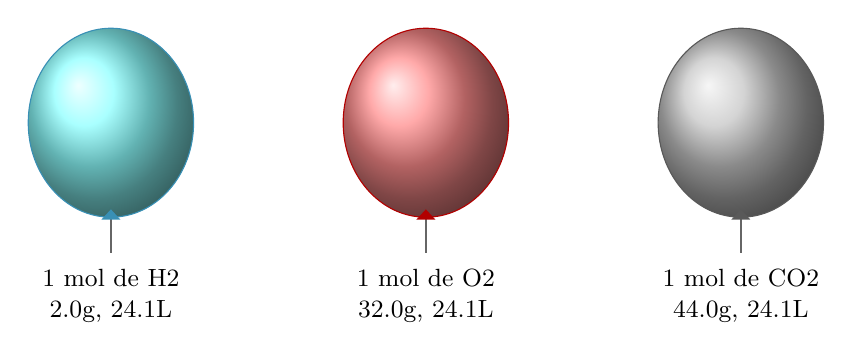
\begin{tikzpicture}[font=\small]
  \foreach \x/\g/\m/\c in {0/{\ce{H2}}/2.0/cyan, 4/{\ce{O2}}/32.0/red,
                           8/{\ce{CO2}}/44.0/gray} {
    \draw[thick, black!60] (\x,-0.25) -- (\x,-1.1);
    \shade[ball color=\c!45, draw=\c!70!black] (\x,0.55) ellipse (1.05 and 1.2);
    \fill[\c!70!black] (\x-0.12,-0.68) -- (\x+0.12,-0.68) -- (\x,-0.55) -- cycle;
    \node[align=center] at (\x,-1.65) {1 mol de \g\\ \qty{\m}{g},
      \qty{24.1}{L}};
  }
\end{tikzpicture}

{\small Três balões a \qty{20}{\celsius}, cada um com um \omterm{def:g10:the-mole:amount}{mol} de um gás
diferente. Os volumes são iguais; as massas não.}
\end{omfigure}


\begin{example}[Um balão de dióxido de carbono]\label{ex:g10:the-mole:balloon}
% ledger: aw:C, aw:O
Um balão contém \qty{2.4}{L} de dióxido de carbono a \qty{20}{\celsius}.
A sua \omterm{def:g10:the-mole:amount}{quantidade de matéria} é
$n = \qty{2.4}{L} / \qty{24.1}{L/mol} = \qty{0.10}{mol}$,
e a sua massa $m = \qty{0.10}{mol} \times \qty{44.0}{g/mol} =
\qty{4.4}{g}$. O mesmo balão cheio de hidrogênio conteria os mesmos
\qty{0.10}{mol}, mas só \qty{0.20}{g} de gás.
\end{example}

\begin{remark}[Gases pesados e gases leves]\label{rem:g10:the-mole:heavy}
Como um litro de qualquer gás contém a mesma \omterm{def:g10:the-mole:amount}{quantidade de matéria}, a
massa de um litro de gás é proporcional à sua \omterm{def:g10:the-mole:molar-mass}{massa molar}. O \omterm{def:g4:air-a-mixture-of-gases:air}{ar}, uma
\omterm{def:g6:pure-substances-and-mixtures:mixture}{mistura} de cerca de quatro quintos de nitrogênio (\qty{28.0}{g/mol}) e
um quinto de oxigênio (\qty{32.0}{g/mol}), se comporta como um gás de
\omterm{def:g10:the-mole:molar-mass}{massa molar} cerca de \qty{29}{g/mol}. Um gás de \omterm{def:g10:the-mole:molar-mass}{massa molar} maior, como
o dióxido de carbono (\qty{44.0}{g/mol}), é mais denso que o \omterm{def:g4:air-a-mixture-of-gases:air}{ar} e se
acumula no fundo de uma adega fechada; um gás de \omterm{def:g10:the-mole:molar-mass}{massa molar} menor, como
o hélio (\qty{4.0}{g/mol}), sobe.
\end{remark}

\section{Exercícios}

\begin{exercise}[$\star$]\label{exo:g10:the-mole:1}
Calcule as \omterm{def:g10:the-mole:molar-mass}{massas molares} do gás oxigênio \ce{O2}, do gás nitrogênio
\ce{N2}, do metano \ce{CH4}, da amônia \ce{NH3} e do dióxido de carbono
\ce{CO2}.
\end{exercise}

\begin{exercise}[$\star$]\label{exo:g10:the-mole:2}
Que \omterm{def:g10:the-mole:amount}{quantidade de matéria} está contida em \qty{36.0}{g} de água? E em
\qty{4.0}{g} de metano?
\end{exercise}

\begin{exercise}[$\star$]\label{exo:g10:the-mole:3}
Qual é a massa de \qty{0.25}{mol} de cloreto de sódio \ce{NaCl}? E de
\qty{2.0}{mol} de dióxido de carbono?
\end{exercise}

\begin{exercise}[$\star$]\label{exo:g10:the-mole:4}
Quantas \omterm{def:g7:atoms-and-molecules:molecule}{moléculas} há em \qty{0.50}{mol} de gás oxigênio? Que quantidade
de ferro contém \num{3.0e24} \omterm{def:g7:atoms-and-molecules:atom}{átomos} de ferro?
\end{exercise}

\begin{exercise}[$\star$]\label{exo:g10:the-mole:5}
A \qty{20}{\celsius} e à pressão atmosférica normal, que volume ocupam
\qty{0.50}{mol} de gás nitrogênio? Que quantidade de gás oxigênio há em
\qty{12}{L} desse gás?
\end{exercise}

\begin{exercise}[$\star\star$]\label{exo:g10:the-mole:6}
Uma gota de água tem volume de \qty{0.050}{mL}, e \qty{1}{mL} de água tem
massa de \qty{1.0}{g}. Quantas \omterm{def:g7:atoms-and-molecules:molecule}{moléculas} de água a gota contém?
\end{exercise}

\begin{exercise}[$\star\star$]\label{exo:g10:the-mole:7}
O que contém mais \omterm{def:g7:atoms-and-molecules:atom}{átomos}, \qty{10}{g} de alumínio ou \qty{10}{g} de
ferro? Explique primeiro sem calcular, e depois verifique calculando.
\end{exercise}

\begin{exercise}[$\star\star$]\label{exo:g10:the-mole:8}
A \qty{20}{\celsius}, calcule a massa de um litro de dióxido de carbono e
a de um litro de gás nitrogênio. Por que o dióxido de carbono se acumula
no fundo de uma adega fechada onde o suco de uva está fermentando?
\end{exercise}

\begin{exercise}[$\star\star$]\label{exo:g10:the-mole:9}
Usando a figura das três caixas $m$, $n$, $N$, dê a massa de
\num{1.0e22} \omterm{def:g7:atoms-and-molecules:molecule}{moléculas} de glicose \ce{C6H12O6}. Anote as duas setas
seguidas.
\end{exercise}

\begin{exercise}[$\star\star$]\label{exo:g10:the-mole:10}
Um cubo de açúcar (sacarose, \ce{C12H22O11}) tem massa de \qty{5.0}{g}.
Calcule a quantidade de sacarose que ele contém, depois o número de
\omterm{def:g7:atoms-and-molecules:molecule}{moléculas} de sacarose, depois o número de \omterm{def:g7:atoms-and-molecules:atom}{átomos} de carbono.
\end{exercise}

\begin{exercise}[$\star\star$]\label{exo:g10:the-mole:11}
O que contém a maior quantidade de \omterm{def:g7:atoms-and-molecules:molecule}{moléculas}: \qty{1.0}{kg} de água
\ce{H2O} ou \qty{1.0}{kg} de etanol \ce{C2H6O}? Por que fator?
\end{exercise}

\begin{exercise}[$\star\star\star$]\label{exo:g10:the-mole:12}
Um anel de ouro tem massa de \qty{5.0}{g}; três quartos da sua massa
são de ouro, o resto de cobre. Quantos \omterm{def:g7:atoms-and-molecules:atom}{átomos} de ouro ele contém?
Quantos \omterm{def:g7:atoms-and-molecules:atom}{átomos} de cobre? Que \omterm{def:g9:periodic-table-first-look:metal}{metal} tem mais \omterm{def:g7:atoms-and-molecules:atom}{átomos} no anel?
\end{exercise}

\begin{exercise}[$\star\star\star$]\label{exo:g10:the-mole:13}
Uma sala de aula mede \qty{8.0}{m} por \qty{6.0}{m} por \qty{3.0}{m}, e
o \omterm{def:g4:air-a-mixture-of-gases:air}{ar} dentro dela está a \qty{20}{\celsius}.
\begin{enumerate}
  \item Que quantidade de gás ela contém ($\qty{1}{m^3} =
        \qty{1000}{L}$)? Quantas \omterm{def:g7:atoms-and-molecules:molecule}{moléculas}?
  \item Tomando o \omterm{def:g4:air-a-mixture-of-gases:air}{ar} como 78 \omterm{def:g7:atoms-and-molecules:molecule}{moléculas} de gás nitrogênio, 21 de gás
        oxigênio e 1 de argônio (\qty{40.0}{g/mol}) em cada cem, calcule
        a \omterm{def:g10:the-mole:molar-mass}{massa molar} média do \omterm{def:g4:air-a-mixture-of-gases:air}{ar}.
  \item Qual é a massa do \omterm{def:g4:air-a-mixture-of-gases:air}{ar} da sala?
\end{enumerate}
\end{exercise}

\begin{exercise}[$\star\star\star$]\label{exo:g10:the-mole:14}
Uma esfera de silício puro tem massa de exatamente \qty{1.000}{kg}.
\begin{enumerate}
  \item Quantos \omterm{def:g7:atoms-and-molecules:atom}{átomos} de silício ela contém?
  \item Deduza a massa de um \omterm{def:g7:atoms-and-molecules:atom}{átomo} de silício.
  \item Antes de 2019, a \omterm{def:g10:the-mole:avogadro}{constante de Avogadro} não era fixada, mas
        medida. Explique como uma contagem independente dos \omterm{def:g7:atoms-and-molecules:atom}{átomos} de uma
        esfera assim, cuja \omterm{def:g10:the-mole:amount}{quantidade de matéria} é conhecida a partir da
        massa, daria um valor para ela.
\end{enumerate}
\end{exercise}

\begin{exercise}[$\star\star\star$]\label{exo:g10:the-mole:15}
% ledger: iso:Cl35, iso:Cl37
O cloro natural contém \qty{75.8}{\percent} de \omterm{def:g7:atoms-and-molecules:atom}{átomos} de cloro-35, de
\omterm{def:g10:the-mole:molar-mass}{massa molar} muito próxima de \qty{35.0}{g/mol}, e \qty{24.2}{\percent}
de \omterm{def:g7:atoms-and-molecules:atom}{átomos} de cloro-37, de \omterm{def:g10:the-mole:molar-mass}{massa molar} muito próxima de
\qty{37.0}{g/mol}. Calcule a \omterm{def:g10:the-mole:molar-mass}{massa molar atômica} do cloro natural e
compare-a com o valor da tabela.
\end{exercise}

\section{Problema: o copo de água de Kelvin}

\begin{problem}[{Problema de fim de semana --- despeje um copo de água no
mar, espere que ele se misture a todos os oceanos e encha de novo um
copo: quantas das primeiras moléculas voltam?}]
\label{pb:g10:the-mole:1}
% ledger: ocean:volume, rho:water, const:NA, aw:H, aw:O
Um experimento mental famoso, muitas vezes atribuído ao físico Lorde
Kelvin, é assim. Marque cada \omterm{def:g7:atoms-and-molecules:molecule}{molécula} de um copo de água, despeje o copo
no mar e espere até que as \omterm{def:g7:atoms-and-molecules:molecule}{moléculas} marcadas tenham se espalhado por
igual por todos os oceanos do mundo. Depois mergulhe o copo no mar de
novo, em qualquer lugar. Ele vai trazer de volta alguma \omterm{def:g7:atoms-and-molecules:molecule}{molécula}
marcada? O copo contém \qty{250}{mL}, e \qty{1}{mL} de água tem massa de
\qty{1.0}{g}. Os oceanos contêm cerca de \qty{1.335e9}{km^3} de água.
Trate a água do mar como água pura para a contagem.

\medskip
\noindent\textbf{Parte I --- A água de um copo.}
\begin{enumerate}
  \item Calcule a \omterm{def:g10:the-mole:molar-mass}{massa molar} da água.
  \item Qual é a massa da água do copo?
  \item Calcule a quantidade de \omterm{def:g7:atoms-and-molecules:molecule}{moléculas} de água no copo.
  \item Que quantidade de \omterm{def:g7:atoms-and-molecules:atom}{átomos} de hidrogênio o copo contém? E de \omterm{def:g7:atoms-and-molecules:atom}{átomos}
        de oxigênio?
\end{enumerate}

\medskip
\noindent\textbf{Parte II --- As \omterm{def:g7:atoms-and-molecules:molecule}{moléculas} do copo.}
\begin{enumerate}[resume]
  \item Quantas \omterm{def:g7:atoms-and-molecules:molecule}{moléculas} de água o copo contém?
  \item Calcule a massa de uma \omterm{def:g7:atoms-and-molecules:molecule}{molécula} de água, em gramas.
  \item Confira as respostas de 5 e 6 multiplicando-as: qual deveria ser
        o produto?
  \item Contando uma \omterm{def:g7:atoms-and-molecules:molecule}{molécula} por segundo, dia e noite, quantos anos
        seriam necessários para contar as \omterm{def:g7:atoms-and-molecules:molecule}{moléculas} do copo? (Um ano dura
        cerca de \qty{3.16e7}{s}.)
\end{enumerate}

\medskip
\noindent\textbf{Parte III --- O oceano.}
\begin{enumerate}[resume]
  \item Converta o volume dos oceanos em metros cúbicos
        ($\qty{1}{km^3} = \qty{e9}{m^3}$), e depois em litros.
  \item Depois que as \omterm{def:g7:atoms-and-molecules:molecule}{moléculas} marcadas se espalharam por igual, quantas
        delas há em cada litro de oceano?
  \item Quantas \omterm{def:g7:atoms-and-molecules:molecule}{moléculas} marcadas o segundo copo traz de volta?
  \item Segundo método. Calcule a quantidade de água dos oceanos, tomando
        \qty{1.0}{kg} como a massa de um litro.
  \item Que fração de todas as \omterm{def:g7:atoms-and-molecules:molecule}{moléculas} de água do oceano está marcada?
  \item Multiplique essa fração pelo número de \omterm{def:g7:atoms-and-molecules:molecule}{moléculas} do segundo copo,
        e compare com a resposta da questão 11.
\end{enumerate}

\medskip
\noindent\textbf{Parte IV --- O que isso significa.}
\begin{enumerate}[resume]
  \item Quantos copos de \qty{250}{mL} poderiam ser enchidos com a água
        dos oceanos?
  \item Compare esse número com o número de \omterm{def:g7:atoms-and-molecules:molecule}{moléculas} de um copo.
        Explique numa frase por que o segundo copo traz de volta tantas
        \omterm{def:g7:atoms-and-molecules:molecule}{moléculas} marcadas.
  \item Que volume de água do mar é preciso tirar, em média, para trazer
        de volta uma única \omterm{def:g7:atoms-and-molecules:molecule}{molécula} marcada? Compare com uma gota de
        \qty{0.05}{mL}.
  \item A resposta da questão 11 tem muitos algarismos. Por que ela só
        deve ser dada como uma ordem de grandeza? Dê duas razões.
  \item Dê a resposta final: mais ou menos quantas \omterm{def:g7:atoms-and-molecules:molecule}{moléculas} do primeiro
        copo voltam no segundo?
\end{enumerate}
\end{problem}
